\documentclass[a4paper, 12pt]{article}
\usepackage{csquotes}
\usepackage{titlesec}
\usepackage[ngerman]{babel}
\usepackage[a4paper, left=3cm, right=3cm, top=2cm, bottom=2cm]{geometry}
\usepackage{fouriernc}
\usepackage{titlesec}
\usepackage{keystroke}

\newcommand{\makeTitleAndTable}{
    \begin{titlepage}
        \centering
        \vspace*{1.5cm}
        {\Huge Einfacher SPH Flüssigkeitssimulator mit Beschleunigter Nachbarschaftssuche\par}
        \vspace{1cm}
        {\LARGE Thierry Meiers\par}
        {\Large Bachelor Projekt\par}
        \begin{figure}[H]
            \centering
            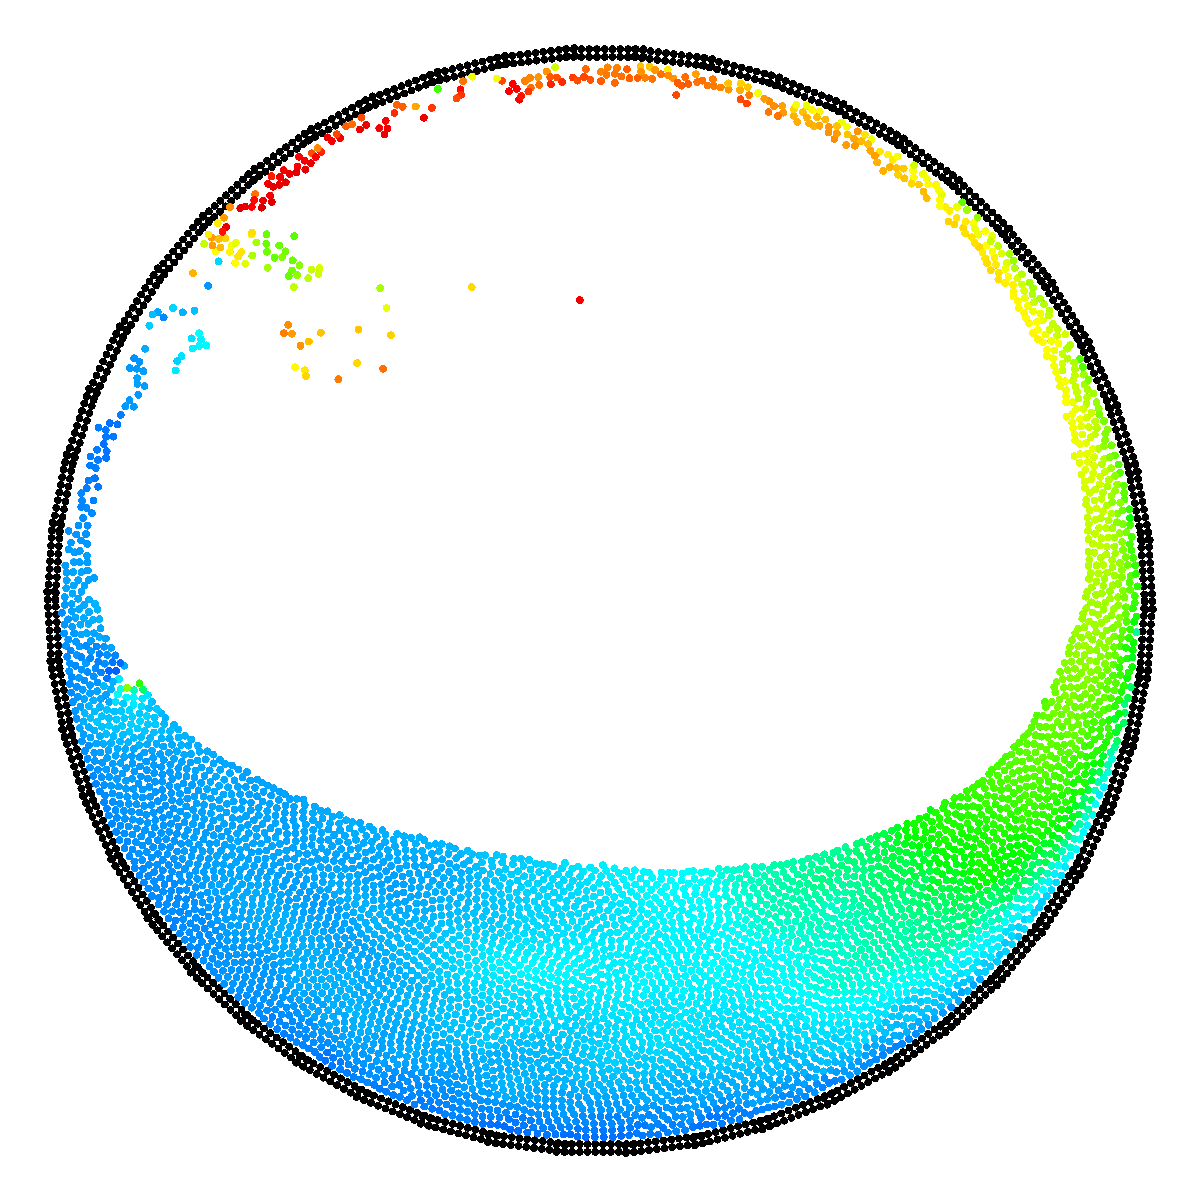
\includegraphics[width=.7\textwidth]{graphics/FirstPage.png}
        \end{figure}
        \vspace{0.5cm}
        {\large Albert-Ludwigs-Universität Freiburg\\Technische Fakultät\\Graphische Datenverarbeitung\par}
        \vfill
        {\large \today \par}
    \end{titlepage}
    \pagenumbering{gobble}
    \tableofcontents
    \clearpage
    \pagenumbering{arabic}
}

\usepackage[ngerman]{babel}
\usepackage[dvipsnames]{xcolor}
\usepackage{graphicx} 
\usepackage{microtype}
\usepackage{subcaption}
\usepackage{float}
\usepackage{parskip}
\usepackage{amsmath}
\usepackage{hyperref}
\usepackage{enumitem}
\begin{document}

\makeTitleAndTable

\section{Einführung}
Fluidsimulationen haben sich zu einem unverzichtbaren Werkzeug in zahlreichen Bereichen unserer Gesellschaft entwickelt. Sie ermöglichen die präzise Simulation von Flüssigkeiten und Gasen in verschiedenen Umgebungen, wodurch das Verhalten dieser Stoffe und ihre Interaktionen mit der Umgebung untersucht werden können. Aufgrund ihrer Vielseitigkeit kommen Fluidsimulationen in einer großen Bandbreite von Anwendungsgebieten zum Einsatz, darunter die Optimierung von Fahrzeugen und Gebäuden, Wettervorhersagen, medizinische Forschung, die Erzeugung realistischer Effekte in Filmen und Spielen, industrielle Prozesse, Energieerzeugung und die Entwicklung von Sportgeräten. Diese Simulationen tragen wesentlich dazu bei, Designs zu verbessern, die Effizienz zu steigern und komplexe Strömungen besser zu verstehen.

Die Allgegenwärtigkeit und Bedeutung dieser Technologie in verschiedenen Branchen haben mein Interesse an diesem Thema geweckt. Insbesondere die Verbindung von Physik und Informatik ist eine Motivation zur Arbeit an diesem Projekt. Das Hauptziel ist die Implementierung der Smoothed Particle Hydrodynamics (SPH) zur Simulation von Fluiden, um ein tieferes Verständnis für die Komponenten und Mechanismen von SPH zu entwickeln. Analysen werden dabei helfen, die Parameter von SPH richtig zu setzen um die Stabilität der Simulation zu optimieren und Fehler in der Implementierung zu finden.

In diesem Bericht werden wir zuerst in Abschnitt \ref{section_1} die Navier-Stokes-Gleichung analysieren, die die Grundlage aller Methoden zur Simulation von Fluiden und Gasen bilden. In Abschnitt \ref{section_2} folgt eine Übersicht aller Teile der SPH-Methode, die zur Implementierung der Simulation verwendet wurden. Wie SPH schlussendlich implementiert wurde, wird in Abschnitt \ref{section_3} beschrieben, zusammen mit einer Übersicht der einzelnen Komponenten. Der wichtigste Teil wird die Analyse und Interpretation der Daten der Simulation in Abschnitt \ref{section_4} sein.

\section{Navier-Stokes-Gleichung} \label{section_1}
Die Navier-Stokes-Gleichungen sind fundamentale Gleichungen in der Fluidmechanik, die das Verhalten von strömenden Flüssigkeiten und Gasen beschreiben. Sie basieren auf den Prinzipien der Erhaltung von Masse, Impuls und Energie. Sie modellieren die Bewegung des Fluids, indem sie die Einflüsse von Druck, Viskosität und externen Kräften auf das Strömungsverhalten berücksichtigen.

\begin{equation}
    \rho(\nabla \vec{v} + (\vec{v} \cdot \vec{\nabla})\vec{v}) = - \vec{\nabla}p + \eta \vec{\nabla}^2 \vec{v} + (\lambda + \eta)\vec{\nabla}(\vec{\nabla} \cdot \vec{v}) + \rho \vec{f}
    \label{equ:Impulsgleichung}
\end{equation} 

Gleichung \eqref{equ:Impulsgleichung} beschreibt die Impulserhaltung. Diese entspricht dem zweitem Newtonsches Gesetz und kann dementsprechend hergeleitet werden:
\begin{align}
    \vec{F}&=\Delta m \cdot a = \Delta m \cdot \nabla \vec{v} \nonumber\\
    \vec{F}&=\rho \cdot \Delta V \cdot \nabla \vec{v} \nonumber\\
    \vec{F}&=\rho \cdot \Delta V (\nabla \vec{v} + (\vec{v} \cdot \vec{\nabla})\vec{v})
    \label{equ:Newtonsches_Gesetz}
\end{align}

Die Masse eines Objektes kann durch $m = \rho * V$ bestimmt werden. Die Geschwindigkeitsänderung ergibt sich aus der Lokalen zeitlichen Beschleunigung $\nabla \vec{v}$ und der Konvektiven Beschleunigung $(\vec{v} \cdot \vec{\nabla})\vec{v}$, also die die Änderung der Geschwindigkeit aufgrund der Bewegung der Flüssigkeit selbst.

Wir benötigen nun die Kräfte $\vec{F}$. Diese sind aus verschiedenen Kräfte welche auf einen Fluid auswirken. Diese bestehen aus der Druck Kraft \eqref{equ:Druck}, der Reibungs Kraft \eqref{equ:Reib}, der Kompressions Kraft \eqref{equ:Kompress} und der Kräfte die von außen wirken \eqref{equ:ext}.

\begin{align}
    \vec{F}_{Druck} &= - \vec{\nabla}p \cdot \Delta V \label{equ:Druck}\\
    \vec{F}_{Reib} &= \eta \vec{\nabla}^2 \vec{v} \cdot \Delta V \label{equ:Reib}\\
    \vec{F}_{Kompress} &= (\lambda + \eta)\vec{\nabla}(\vec{\nabla} \cdot \vec{v}) \label{equ:Kompress}\\
    \vec{F}_{ext} &= \rho \vec{f} \cdot \Delta V \label{equ:ext}
\end{align}

\begin{equation} \label{equ:Kraft}
    \vec{F} = \vec{F}_{Druck} + \vec{F}_{Reib} + \vec{F}_{Kompress} + \vec{F}_{ext}
\end{equation}

Wir setzen \eqref{equ:Kraft} in die Gleichung \eqref{equ:Newtonsches_Gesetz} ein und erhalten somit:

\[- \vec{\nabla}p \cdot \Delta V + \eta \vec{\nabla}^2 \vec{v} \cdot \Delta V + \rho \vec{f} \cdot \Delta V = \rho \cdot \Delta V (\nabla \vec{v} + (\vec{v} \cdot \vec{\nabla})\vec{v})\]

Durch das dividieren beider Seiten mit $\Delta V$ erhält man schließlich die Gleichung \eqref{equ:Impulsgleichung}.

\[- \vec{\nabla}p + \eta \vec{\nabla}^2 \vec{v} + \rho \vec{f} = \rho (\nabla \vec{v} + (\vec{v} \cdot \vec{\nabla})\vec{v})\]

Des weiterem folgt die Kontinuitätsgleichung welche die Erhaltung der Masse innerhalb eines Fluides beschreibt. 

\begin{equation} \label{equ:Kontinuitätsgleichung}
    \Delta \rho + \vec{\nabla} \cdot (\rho \vec{v}) = 0
\end{equation}

In ihrer klassischen Form sind sowohl die Impulsgleichung \eqref{equ:Impulsgleichung} als auch die Kontinuitätsgleichung \eqref{equ:Kontinuitätsgleichung} spezifisch für Newtonsche Fluide formuliert. Newtonsche Fluide zeichnen sich durch ein lineares viskoses Fließverhalten aus, bei dem die Viskosität unabhängig von der Schergeschwindigkeit ist.

\section{Smoothed Particle Hydrodynamics} \label{section_2}

\section{Implementierung} \label{section_3}
\subsection{Simulation}
\subsection{Nachbarschaft Suchen}
\subsection{Oberflächenspannung}

\section{Analysen} \label{section_4}

\section{Schlussfolgerung}

\section{Bibliographie}
\end{document}